\documentclass[journal]{IEEEtran} 

\pdfoutput=1

\usepackage[T1]{fontenc}
\usepackage[latin9]{inputenc}
\usepackage{verbatim}
\usepackage{float}
\usepackage{amsthm}
\usepackage{amsmath}
\usepackage{amssymb}
\usepackage{graphicx}
%\usepackage{multirow}
\usepackage{color}
\usepackage{url}

\usepackage{algorithm}

\newcommand{\TODO}[1]{{\color{red}{[#1]}}}

\makeatletter


%%%%%%%%%%%%%%%%%%%%%%%%%%%%%% Textclass specific LaTeX commands.
\numberwithin{equation}{section}
\numberwithin{figure}{section}
\theoremstyle{plain}
\newtheorem{thm}{\protect\theoremname}[section]
\theoremstyle{definition}
\newtheorem{defn}[thm]{\protect\definitionname}
\theoremstyle{remark}
\newtheorem{claim}[thm]{\protect\claimname}
\theoremstyle{plain}
\newtheorem{lem}[thm]{\protect\lemmaname}

\newtheorem*{lem*}{Lemma}
\theoremstyle{remark}
\newtheorem{rem}[thm]{\protect\remarkname}
\theoremstyle{plain}
\newtheorem{corollary}[thm]{\protect\corollaryname}
\theoremstyle{plain}
\newtheorem{proposition}[thm]{\protect\propositionname}
%%%%%%%%%%%%%%%%%%%%%%%%%%%%%% User specified LaTeX commands.

%\usepackage{babel}
\providecommand{\claimname}{Claim}
\providecommand{\definitionname}{Definition}
\providecommand{\lemmaname}{Lemma}
\providecommand{\remarkname}{Remark}
\providecommand{\theoremname}{Theorem}
\providecommand{\corollaryname}{Corollary}
\providecommand{\propositionname}{Proposition}


\newcommand{\RL}{\mathbb{R}^L}
\newcommand{\RN}{\mathbb{R}^N}
\newcommand{\CL}{\mathbb{C}^L}
\newcommand{\CN}{\mathbb{C}^N}
\newcommand{\RW}{\mathbb{R}^W}
\newcommand{\RNN}{\mathbb{R}^{N\times N}}
\newcommand{\CNN}{\mathbb{C}^{N\times N}}
\newcommand{\inner}[1]{\left\langle {#1} \right\rangle}
\newcommand{\E}[1]{\mathbb{E}\left\{{#1} \right\}}
\newcommand{\order}[1]{\mathcal{O}\left({#1} \right)}
\newcommand{\xz}{x_{\textrm{zp}}}
\newcommand{\DFT}{\operatorname{DFT}}
\newcommand{\SNR}{\operatorname{SNR}}
\newcommand{\hx}{\hat{x}} 


\begin{document}

%\begin{frontmatter}


\title{Multireference alignment meets blind deconvolution}
\author{Tamir Bendory}
\maketitle

\begin{abstract}
	Here comes the abstract
\end{abstract}

\begin{IEEEkeywords}
	Blind deconvolution, multireference alignment, bispectrum, cryo-EM
\end{IEEEkeywords}


\section{Introduction} \label{sec:introduction}

Blind deconvolution is a longstanding problem, arising in a variety of engineering and scientific applications, such as astronomy, communication, image deblurring, system identification and optics; see   \cite{jefferies1993restoration,tong1994blind,chan1998total,campisi2016blind,kundur1996blind,levin2011understanding,shalvi1990new,levin2009understanding,krishnan2011blind,ayers1988iterative,michaeli2014blind,lin2005relevant,abed1997blind}, just to name a few. In blind deconvolution, we aim at estimating  a signal from its convolution with an unknown kernel. 
Clearly, without additional information, the problem is ill-posed.

In this paper, we consider a particular case, in which one signal is of finite support, while the other is a binary sparse signal. Let us define the (zero-padded) signal 
$$\xz  = [x, \underbrace{0,0,\ldots,0}_{N-L \text{ zeros}}]\in\RN,\quad N\gg L,$$
and a binary signal $s\in\{0,1\}^N$. Then, our goal is to estimate $x$ from \begin{equation} \label{eq:blind_deconvolution}
y = \xz \ast s + \varepsilon,
\end{equation}
where $\varepsilon$ is an i.i.d.\ normal noise $\varepsilon$ with mean zero and variance $\sigma^2$.
As can be seen, the measurement $y\in\RN$ is composed of repetitions of an underlying signal $x\in\RL$, located at different positions. So, we can also write the model as  
\begin{equation}
y[n] = \sum_{i=1}^K \xz [n-n_i] + \varepsilon[n], 
\end{equation}
where the $n_i$'s are the non-zero values of $s$.

While most works on blind deconvolution tries to estimate both unknown signals (see Section~\ref{sec:blind_deconvolution}), in most cases, the goal is merely to estimate one of the signals.
For instance, in image deblurring, both the blurring kernel and the high-resolution image are unknown, but the main goal is only to sharpen the image. In~\eqref{eq:blind_deconvolution}, the signal $s$ is referred to as the latent or hidden variable of the problem. Our goal is to estimate  $x$ and we focus  on the low signal--to--noise ratio ($\SNR$) regime. As will be demonstrated, in this case, estimating $s$ is impossible, even if $\xz$ is known. However, we show, maybe surprisingly, that one can estimate $x$ accurately in some cases.  We support this statement by theoretical analysis and numerical  experiments.

Figure~\ref{fig:example} shows examples of the problem in different noise levels. In the example, the signal $x$ appears twice in $y$ so that $\| s \|^2 = 2$. The first row demonstrates a high $\SNR$ regime with $\sigma = 0.1$. As can be seen, in this regime  the problem is rather easy. In this case, one can easily the support of $s$ (namely, the repetition of $x$ in $y$) by simple detection algorithms. This is demonstrated by the correlation function between $\xz$ and $y$ that exhibits two unmistakable peaks in the support of $x$.  Once several copies of the signal were detected and cropped from $y$, then one can  improve the $\SNR$ by averaging. We are interest in the more challenging regime of high noise level, as exemplified in the bottom row ($\sigma  = 3$)
in which the signal is completely swamped in the noise, and one cannot detect the signal's appearances. In this case, one need to use the prior information that the signal appears many times across the measurement.

\begin{figure*}
	\begin{center}
	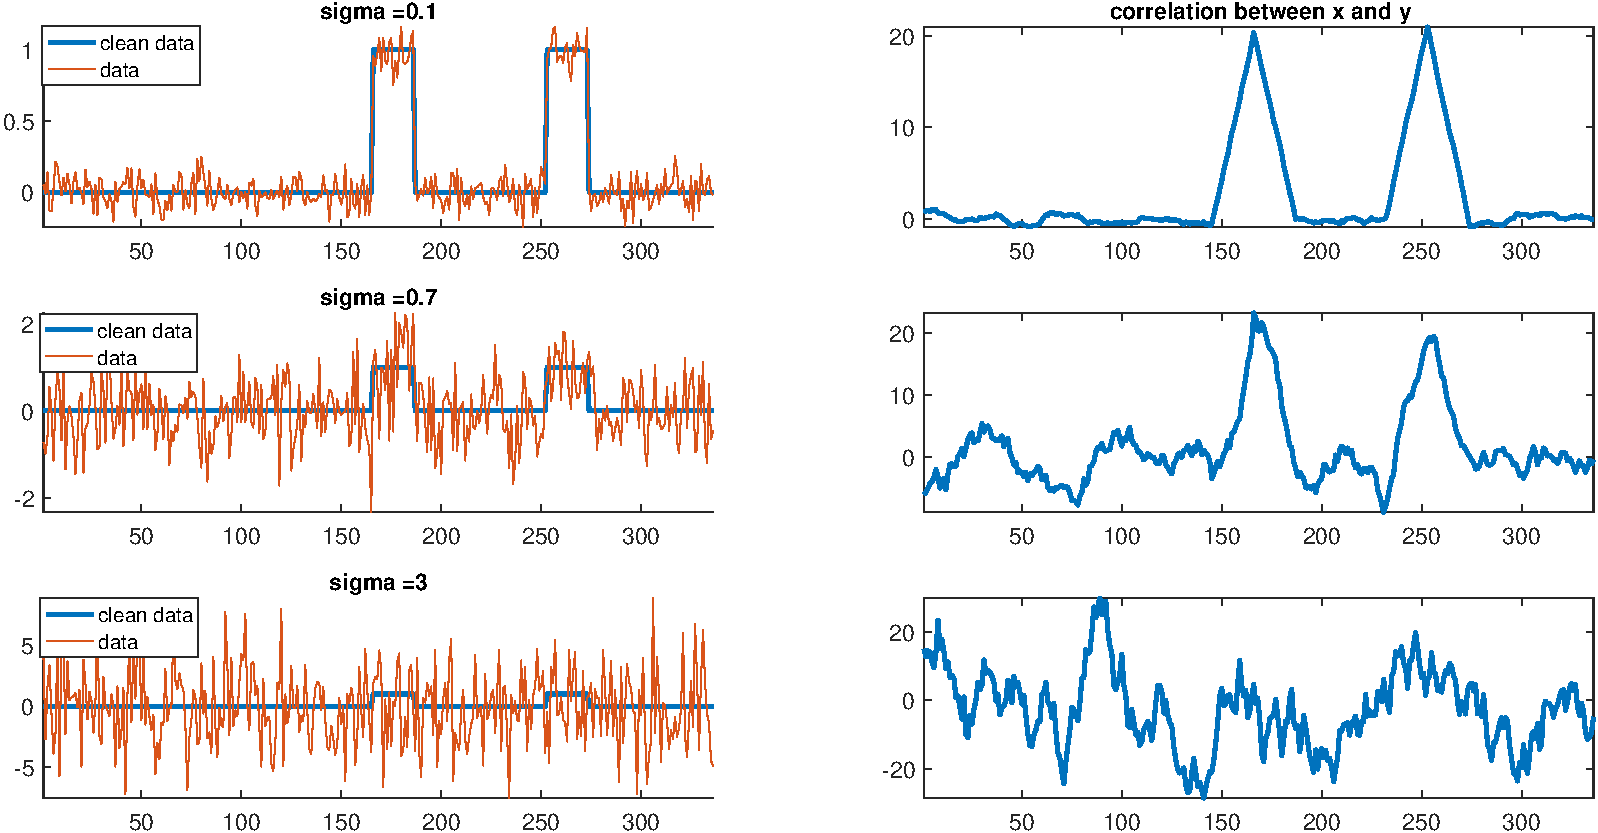
\includegraphics[scale = .5]{example}
	\end{center}
\caption{The left column presents the clean data and the measurement in different noise levels. In this example, a rectangular signal of length $L=21$ appears twice in a measurement of length $N=336$ with different noise levels. Note to the different scale of the y-axis. The right column presents the correlation between the rectangular signal and the measurement for the associated problems. }
\label{fig:example}
\end{figure*}

Our approach for this blind deconvolution problem is based on  tools that were developed for the multireference alignment (MRA) problem. MRA is the problem of estimating a signal from its circularly-shifted noisy measurements~\cite{bandeira2014multireference,bendory2017bispectrum} 
 In Section~\ref{sec:mra}, we survey recent works in this field. We use a recent suggestion to estimate the signal from feature that are invariant under cyclic-translation~\cite{bendory2017bispectrum}. 
 In essence, our method is based on \emph{approximate reduction} of the blind deconvolution problem into the MRA model. This is done be splitting $y$ into shorter windows and treat them as the MRA measurements. If each window contains exactly  one signal, then the problem reduces exactly the MRA problem. However, this is not the case. Some windows contain only noise, while others contain both noise and parts of a signal.  
 We analyze the estimation rate of this method and its deviation from the MRA model. 
 
 A motivation for this work arises from the cryo--electron microscopy (EM) problem. Cryo--EM received a great deal of attention in structural biology in recent years as it allows visualizing molecules that were not stained in any way, showing them in their native environment. In Section~\ref{sec:cryoEM} we draw the connections between  blind deconvolution and the cryo--EM problem.
 
 The outline of this paper is as follows. In Section~\ref{sec:literature} we introduce background  on blind deconvolution (Section~\ref{sec:blind_deconvolution}) and MRA (Section~\ref{sec:mra}).  
 In Section~\ref{sec:cryoEM} we discuss the connection with the  cryo--EM problem.  In Section~\ref{sec:algorithm} we introduce the algorithm and analyze it in Section~\ref{sec:analysis}. Section~\ref{sec:experiments} is devoted for numerical experiments. Section~\ref{sec:conclusion} concludes the manuscript.
 



\section{background} \label{sec:literature}

In this section, we introduce the two main ingredients of this work, blind deconvolution and MRA. Then, we draw connections  with the cryo--EM problem.

\subsection{Blind deconvolution} \label{sec:blind_deconvolution}


Blind deconvolution is the problem of recovering a signal from its convolution with an unknown kernel $h$. That is, we aim to recover  $x$ from
\begin{equation}
y = x\ast h,
\end{equation}
where both $x$ and $h$ are unknown. In the Fourier domain, it takes the form of 
\begin{equation}
Fy = Fx \odot Fh,
\end{equation}
where $Fz$ stands for the Fourier transform of $z$ and $\odot$ for entry-wise product.
Clearly, without prior information of the signal, it is impossible to estimate the signal. For instance, even if we assume that the $\DFT$ of both signals are non-vanishing, then $Fy$ remains unchanged if we replace $(Fx)[k],(Fh)[k]$ by $a(Fx)[k],\frac{1}{a}(Fh)[k]$ for any $a\in\CN\backslash\{0\}$ and any $k$.


The blind deconvolution  has been analyzed recently with a various convex and non-convex algorithms. These works assume that the signal lies in a known  subspace spanned by vectors with random entries~\cite{ahmed2014blind,li2016rapid,ling2017blind}. A somewhat more related line of works assume sparsity in a random linear subspaces~\cite{lee2017blind,ling2015self,chi2016guaranteed}. 
The papers 
\cite{choudhary2014sparse,li2016identifiability,kech2017optimal,li2015unified} deals with the fundamental question of identifiability of the problems, but none of these paper consider our setup, namely, when the sparse signal is in the canonical basis. 

Our problem is very different from all previous works in at least two ways. First, 
while we do assume that one of the signals is sparse,  our goal is to estimate the other signal. We do not claim that we can estimate the sparse signal. Second, we are mainly care of accurate estimation of $x$ in the low $\SNR$ regime. In this regime, it seems that estimating the sparse signal $s$ is impossible. This is contrast to previous works that focused on the high $\SNR$ regime.

We briefly mention that the deconvolution problem, namely, when the kernel is assumed to be known, has been analyzed throughly in recent years under sparsity constraints~\cite{bendory2016robust,bendory2017robust,bendory2016stable,boyer2017adapting,bernstein2017deconvolution,de2012exact,azais2015spike,duval2015exact,duval2015sparse}.  Nevertheless, the problem under consideration is essentially different  from two reasons. First, of course, we consider the blind setting when the kernel is unknown. Second, these works considered the recovery of sparse signal, with Gaussian-like kernel. In our problem, the convolution itself kernel is sparse, while we aim to recover a general signal. 
. 


\subsection{Multireference alignment} \label{sec:mra}

Our approach for blind deconvolution is based on reducing the problem, approximately, to an MRA problem.
In MRA, we aim at estimating a signal $x\in\RL$ from its circularly shifted noisy measurements
\begin{equation} \label{eq:mra}
y_j = R_{r_j}x + \varepsilon_j, \quad j = 1,\ldots,N,
\end{equation}
where $R_{r}$ translates a signal by $r$ locations, namely, $(R_rx)[i] = x[(i-r)\mod L]$, and $\varepsilon$ is an i.i.d.\ normal noise with mean zero and variance $\sigma^2$. This problem finds applications in radar, image processing and structural biology~\cite{zwart2003fast,foroosh2002extension,diamond1992multiple}. The algorithmic and statistical characterizations of this problem have been analyzed thoroughly in the last couple of years, see~\cite{bendory2017bispectrum,bandeira2014multireference,bandeira2017optimal,perry2017sample,boumal2017heterogeneous,abbe2017multireference,abbe2017sample}.

In this work, we exploit the algorithmic framework proposed in~\cite{bendory2017bispectrum}. In order to estimate the signal, this paper suggests to use features of the signal that are invariant under cyclic translation.
Apparently, three moments are required. The first is mean of the signal, denoted by $\mu_x$, or, equivalently, it DC component $(Fx)[0]$. The second feature is the power spectrum of the signal $P_x[k] = \vert (Fx)[k]\vert^2$ for $k=0,1,\ldots L-1$. Since in general one cannot estimate  a signal from its power spectrum~\cite{bendory2017fourier}, one needs a third order feature. This third order feature, called bispectrum, is defined as~\cite{tukey1953}
\begin{equation}
B_x[k_1,k_2] = (Fx)[k_1]\overline{(Fx)[k_2]}(Fx)[k_2-k_1].
\end{equation}  
These features can be estimated directly from the measured data by
\begin{align} \label{eq:moment_estimation}
\frac{1}{N}\sum_{i=1}^N\mu_{y_j}  &\,\to \, \mu_x, \nonumber\\
\frac{1}{N}\sum_{i=1}^NP_{y_j}  &\,\to \, P_x + L\sigma^2, \\
\frac{1}{N}\sum_{i=1}^NB_{y_j}  &\,\to \, B_x + \mu_x\sigma^2L^2A,  \nonumber
\end{align} 
where $A$ is a known deterministic matrix. Therefore, by proper debiasing, one can get a reliable estimating of these features. For large enough $\sigma$, the variance of the estimators  is dominated by the bispectrum and thus goes as $\sigma^6/N$. This estimation rate is optimal under the assumption that distribution of translations is uniform~\cite{bandeira2017optimal}. If the distribution is non-uniform, then one can do better using only the first two moments, see~\cite{abbe2017multireference}. 
 Given enough measurements, one can obtain reliable estimation of the features, and then to estimate the underlying signal, up to cyclic translation, using a variety of algorithms~\cite{bendory2017bispectrum}. In this work, we use a simple non-convex least-squares estimator.... \TODO{Need to see what do we actually solve...}




\subsection{Connections with the cryo--EM problem} \label{sec:cryoEM}

This work is partially motivated by the imaging
technique called single particle cryo--EM, enabling the visualization of molecules at near atomic resolution~\cite{bartesaghi20152,sirohi20163}. Cryo--EM gained a lot of popularity in recent years in the structural biology community. As a result, Dubochet, Frank and Henderson were recently awarded the 
the Nobel prize for their contribution in the development of this technique~\cite{nobel}. 

In cryo--EM, many samples of a molecule are frozen in a thin sheet of ice. 
An electron beam then passes through the ice and the samples  and recorded by an array of detectors. Cryo--EM contains several such images, which are
called \emph{micrographs}. Each micrograph  contains many two-dimensional (2D) tomographic projections of the samples. 
 The  cryo--EM problem is then to estimate the molecules from the micrographs. This process is illustrated by in Figures~\ref{fig:cryo-EM} and~\ref{fig:cryo-EM-problem}. 

Compared to more traditional tomographic methods, like computerized tomography (CT), the cryo--EM problem arises two main challenges. First, the 3D orientation of each sample is unknown since the samples are rapidly frozen in the ice sheet. The experimentalist does not have control over these orientations. Second, the $\SNR$ in each projection is very low since the electron dosage must be restricted to limit  radiation damage to the molecules. In real cryo--EM data sets, there are some additional challenges, like the contrast transfer function of the microscope that corrupts the acquired image. 


\begin{figure}
	\begin{center}
		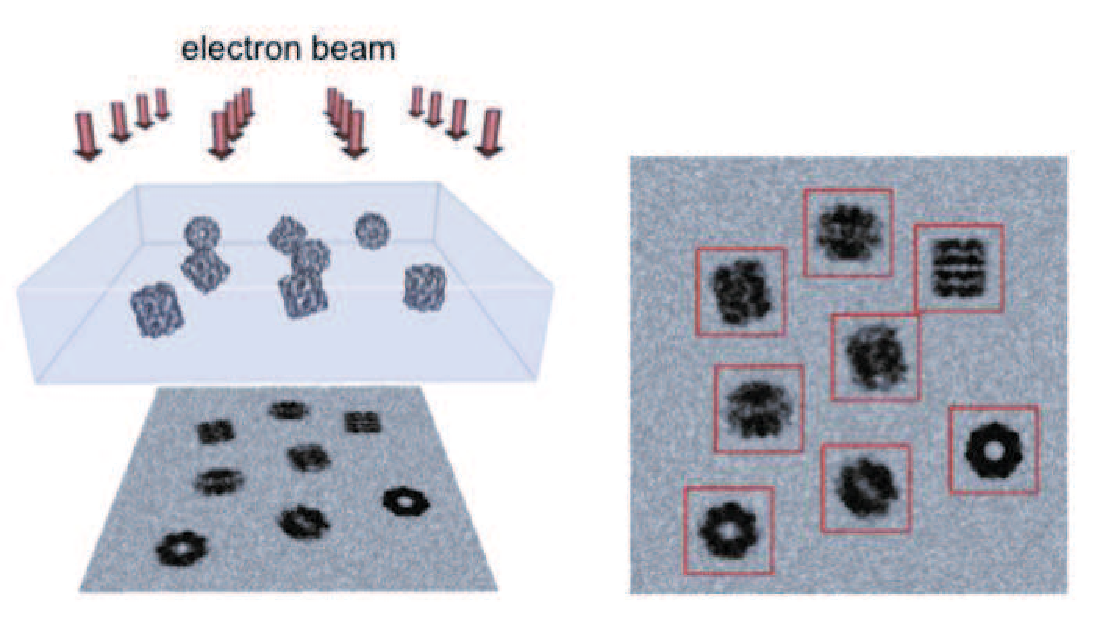
\includegraphics[scale = .4]{cryoem-eps-converted-to}
	\end{center}
	\caption{A schematic draw of the micrograph generation. Courtesy of ?}
	\label{fig:cryo-EM}
\end{figure}

\begin{figure}
	\begin{center}
		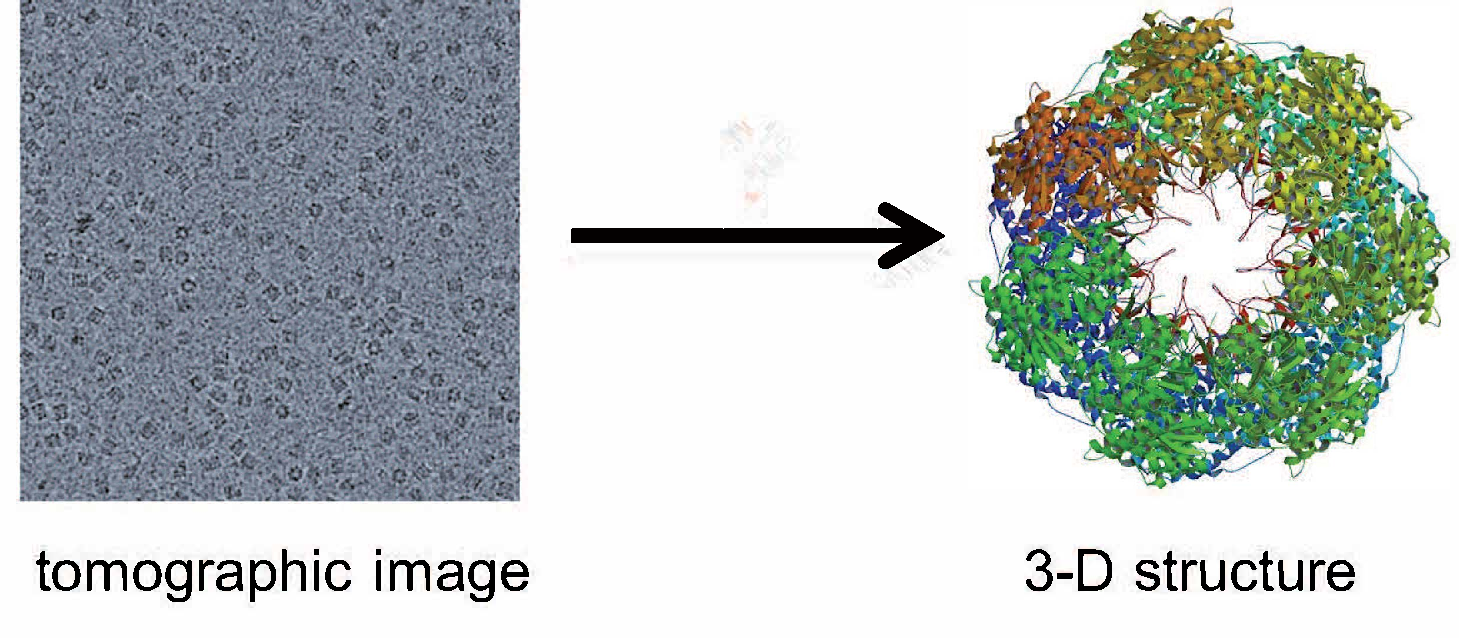
\includegraphics[scale = .35]{cryoem-problem-eps-converted-to}		
	\end{center}
	\caption{The cryo--EM problem: estimating a molecule from the micrograph. Courtesy of ?}
	\label{fig:cryo-EM-problem}
\end{figure}

The first stage of a cryo--EM reconstruction algorithm is the so called \emph{particle picking} stage. In this stage, the projections are detected in the micrographs, and then cropped to a series of 2D images.  Many algorithms were proposed to this detection problem based on support vector machine classifiers, deep learning and template matching and more; see for instance \cite{frank1983automatic,scheres2015semi,arbelaez2011experimental,zhu2016deep}.
 The most popular techniques are based on the latter, where the templates can manually or automatically selected.  The underlying idea is that the cross-correlation  should be high in the presence of a signal in the template. However, this is not true anymore in the presence of high noise level, even if the signal itself is known, as demonstrated in Figure~\ref{fig:example}. An illuminating examples are given in~\cite{shatsky2009method,bandeira2015non}, where the famous picture of Albert Einstein is used to match pure noise and rotated images of the mathematician  Hermann Weyl.
 
 
After the particle picking, ideally, one gets a set of measurements of the form 
\begin{equation} \label{eq:cryo-em}
y_j = \mathcal{P}( g_j\circ x) + \varepsilon_j,\quad j=1,\ldots,N, 
\end{equation}
where $x$ is the three-dimensional (3D) molecule to be estimated,  $g_j\in SO(3)$ are unknown 3D rotations that act on the molecule and $\mathcal{P}$ is a linear tomographic projection. This model has been analyzed theoretically from different point--of-views~\cite{bandeira2015non,hadani2011representation}. The MRA model~\eqref{eq:mra} can be interpreted as a simplification of the model~\eqref{eq:cryo-em}, where the unknown cyclic-shifts correspond to the unknown rotations (but there is no analog for the projection operation).

In practice, particle picking algorithms are far from being optimal, mainly because the high noise level prevents reliable detection. One result is that the cropped images are usually not centered,  and therefore an unknown 2D translation should be added to the model~\eqref{eq:cryo-em}.
In addition, many samples in the micrograph are non detected or ignored.
After the particle picking stage, the molecule is estimated from the 2D images, where the most popular algorithms are based on expectation--maximization (see for instance~\cite{scheres2012relion}). Other techniques, such as the common-lines\cite{van1987angular,singer2011three} method or auto-correlation analysis~\cite{kam1980reconstruction,levin20173d}, can be used for ab initio modeling. 
 
 Our model can be seen as a highly simplified cryo--EM model, where $y$ corresponds to the micrograph and the signal repeated $x$ to a  ``one-dimensional molecule" (the tomographic projection $\mathcal{P}$ does not appear in the model). We are interest in the question whether we can estimate the signal $x$, even if the $\SNR$ is so low that we cannot detect the locations of $x$, in $y$. In the perspective of the cryo--EM problem. the success to estimate the signal in the very low SNR regime may indicate that the molecule can be estimated directly from the cryo--EM micrographs, even if the SNR is so low that particle picking algorithm work poorly. 

  %In addition, most particle picking algorithms throw away many particles since they fail to detect them. Hence, a necessary condition for the success of such algorithm is that the noise level would low enough so that detection would be possible.


   

\section{Algorithm} \label{sec:algorithm}

The blind deconvolution algorithm is inspired by the recent MRA approach using translation invariant features proposed in~\cite{bendory2017bispectrum}. The algorithm requires setting a parameter $W\in\mathbb{N}$ obeying $W>L$  which is the length of the \emph{analysis window}. We assume henceforth, to ease notation, that $W$ divides $N$. 
The algorithm begins with splitting the measurement $y\in\RN$ into a series of analysis windows $y_i\in\mathbb{R}^W,\,i=1,\ldots,N/W$, where  
\begin{equation} \label{eq:analysis_window}
y_i[n] = y[(i-1)W + n] , \quad n=1,\ldots,W. 
\end{equation}
By assumption, there are exactly $N/W$ windows. Of course, one can easily modify the algorithm using overlapping windows, however, our numerical experiments indicate it does not improve the numerical performance.  For each window, we then compute its first three translation-invariant features, namely, mean, power spectrum and bispectrum, and then  average them over all windows according to~\eqref{eq:moment_estimation}
Following~\eqref{eq:moment_estimation}, we estimate the features of the signal by average over the features of the analysis windows, namely,
\begin{align} \label{eq:estimated_features_win}
\hat{\mu}_{x} &= \frac{W}{N}\sum_{i=1}^{N/W}\mu_{y_i}, \\ \nonumber
\hat{P}_{x} &= \frac{W}{N}\sum_{i=1}^{N/W}P_{y_i} - L\sigma^2, \\
\hat{B}_{x} &= \frac{W}{N}\sum_{i=1}^{N/W}B_{y_i-\hat{\mu}_{x_W}}.  \nonumber
\end{align}
As discussed in~\cite{bendory2017bispectrum}, we can replace the mean by more robust estimator, like the median.
 Finally, once we estimated these features, we look for a signal $\hat{x}\in\mathbb{R}^W$ that is consistent with the data by solving ??

Recall that the current estimate $\hat{x}$ is a signal of length $W$, whereas the underlying signal of length $L$.
Ideally, it is cyclic-shifted version of $x$, padded with $W-L$ zeros.
 To crop the signal correctly, we simply search for the  segment of length $L$ with maximal energy. Formally, let  $T_\ell:\RW\to\RL$ be the operator that takes $L$ consecutive entries of the signal, starting at $\ell$. The signal is treated as periodic.   
Then, by letting
\begin{equation}
\ell_{\max} =  {\arg\max}_{\ell=0,\ldots,W-1} \|T_\ell\hat{x} \|_2,
\end{equation}
we map
\begin{equation} \label{eq:align}
\hat{x}\gets T_{\ell_{\max}}\hat{x}.
\end{equation}


The scaling of $\hat{x}$ is incorrect, since the averaging in done over many windows containing pure noise with no information on the signal itself. 
To rescale the estimated signal, we estimate the norm of the signal separately.
The norm estimation can be done as follows. For short, we denote $x_K[n]=\sum_{i=1}^K \xz[n-n_i]$ and note that $\|x_K\|_2^2 = K\|x\|_2^2$ if a separation of $\vert n_i - n_j\vert >L$ is satisfied. 
Then,
\begin{equation}
\| y\|_2^2 =  \| x_K\|_2^2 + \|\varepsilon\|_2^2 + 2\varepsilon^Tx_K, 
\end{equation}  
and therefore 
\begin{equation}
\begin{split}
\E{\| y\|_2^2} &=  \| x_K\|_2^2 + \E{\|\varepsilon\|_2^2} + 2\E{\varepsilon^Tx_K} \\ 
&= K\|x\|_2^2 + N\sigma^2. 
\end{split}	 
\end{equation}   
As $N\to\infty$,  we then obtain
\begin{equation} \label{eq:norm_estimation}
\|x\|_2^2 \approx \frac{\| y\|_2^2 - N\sigma^2}{K}. 
\end{equation}
The estimation error for different values of $\sigma$ is depicted in Figure~\ref{fig:norn_error}. 

\begin{figure}
	\begin{center}
		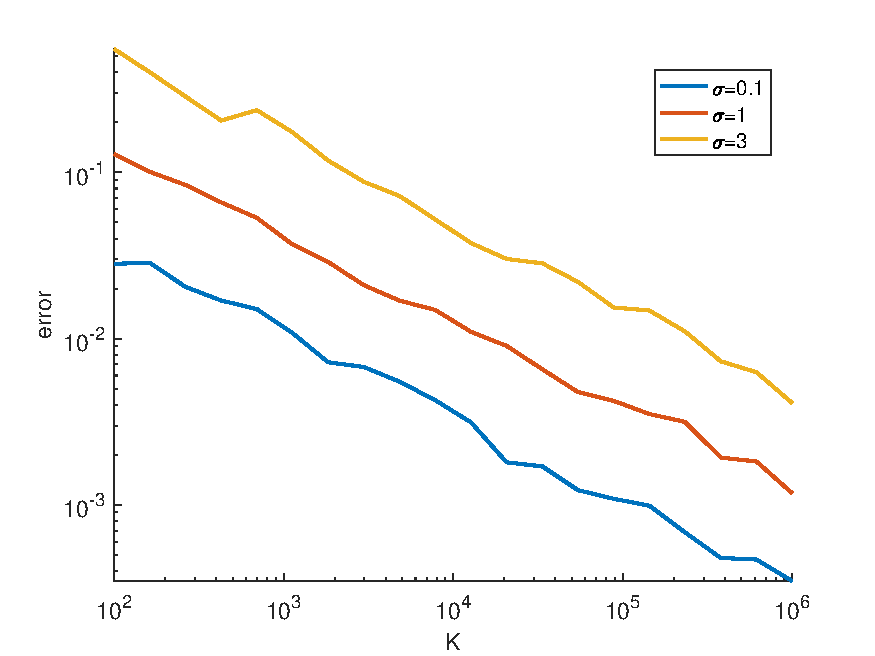
\includegraphics[scale = .5]{NormError}		
	\end{center}
	\caption{The normalized error for norm estimation $\frac{\vert \|\hat{x}\|  - \|x\|\vert }{\|x\|}$, where $\|\hat{x}\|$ is the norm estimation. The error was averaged over 200 experiments for each value of $k$.}
	\label{fig:norn_error}
\end{figure}

The output of the algorithm is a signal of length $W$, that, ideally, contains $x$, shifted by some unknown shift, and padded by $W-L$ zeros. 
The algorithm is summarized in Algorithm~\ref{alg:1}.


\begin{algorithm}[h]
		\textbf{Input:} The measurement $y\in\RN$ \\ 
		\textbf{Output:} A signal $\tilde x\in\mathbb{R}^W$  \\ 
		\begin{enumerate}
			\item Split $y$ into a set of $N/W$ analysis windows $y_i\in\mathbb{R}^W$ according to~\eqref{eq:analysis_window}
			\item  Compute the average mean, power spectrum and bispectrum according to~\eqref{eq:moment_estimation} 
			\item  Estimate the signal $\hat{x}\in\mathbb{R}^W$ by~?
			\item  Map $\hat{x}\gets T_{\ell_{\max}}\hat{x}$ according to~\eqref{eq:align}
			\item  Compute the estimated norm $x_{\textrm{norm}}$  by~\eqref{eq:norm_estimation}
			\item  Rescale the signal $\tilde x \gets \frac{\tilde{x}\cdot x_{\textrm{norm}}}{\|\tilde{x}\|_2} $   
		\end{enumerate}
	\caption{Blind devolution by invariant features} 	\label{alg:1}
\end{algorithm}


\section{Analysis} \label{sec:analysis}

In this section, we analyze the performance of Algoritmh~\ref{alg:1}. Our analysis is based on the asymptotic regime in which  $N,\sigma,K\to\infty$ and  $L,W$ are fixed. Since we work in high noise regime, We focus on the converges rate of the noise terms. In addition, we analyze the error occurred due to the proposed technique independent of the noise.
 We assume that positions $n_i$ are well-separated so that $\vert n_i - n_j\vert >2W$. The factor 2 is merely to ease the analysis is not really required by the algorithm. We also assume that each $n_i$ is uniformly distributed within the window. 


Our framework is based on splitting the measurement into $N/W$ windows $y_i\in\RW$. Since in the high noise regime, we cannot detect the appearances of the signal in $y$, the devision is somewhat arbitrary. The windows $y_i,\,i=1,\ldots,N/W$ can be classified into three classes.  The first class contains a signal in an unknown location and noise. These are ``good" windows since they are perfectly match the MRA model. The second class contains only noise -- no signal.  As will be demonstrated, these windows cause only a scaling problem which is easily fixed by estimation the signal's norm separately~\eqref{eq:norm_estimation}. The third class of signals contains only part of a signal and the noise. These are the ``bad" windows, as they do not contain the entire information of the signal, but, also, do not obey the Gaussian statistics of the noise. These windows induce estimation error, independently of the noise.  

The performance of the algorithm relies on the factors.  The first is the ratio between the length of the analysis window and the signal, namely, 
$$P := W/L>1.$$ Clearly, the larger this ratio is, the less windows are with the class of ``bad" windows; the windows with part of the signal.  On the other hand, if we impose large $P$, we restrict ourselves to work with very sparse signals. The second factor is defined as $$S = \frac{N}{WK},$$ where $WK$ is a measure for the ``active" windows. We refer to $S$ as the  ``sparsity factor". Clearly,  $1<S<\infty$. The larger $S$ is, the more sparse the signal is.


Let us define  the zero padded signal $$x_W  = [x, \underbrace{0,0,\ldots,0}_{N-W \text{ zeros}}]\in\mathbb{R}^W.$$ 
We want to estimate the features of this signal from the features of the $y_i$'s.
In Algorithm~\ref{alg:1} there is another step of trimming this padded signal to a shorter signal of length $L$ that contains most of the information, but we currently ignore this stage. 
 
We next analyze the estimation error of the invariant features, estimated by~\eqref{eq:estimated_features_win}.  
In the ideal case, when one has $n$ windows with signal and noise, them  the asymptotic  estimation rate of the mean, power spectrum and bispectrum is $\sigma^2/n,\,\sigma^4/n,\,\sigma^6/n$, respectively. We are interest in how this rate is changed in the model under consideration.

For each feature, the sum in~\eqref{eq:estimated_features_win} can be split into three classed. For instance, the estimated bispectrum can be written as
\begin{eqnarray}
\hat{B}_{x_W} = B_\textrm{signal} + B_\textrm{clutter} + B_\textrm{noise}, 
\end{eqnarray}
where
\begin{itemize}
	\item $B_\textrm{noise}$ - sum of the bispectra of the segments that contain pure noise (no signal),
	\item $B_\textrm{signal}$ - sum of the bispectra of the segments that contain a full signal (one appearance of $x$) and noise,
	\item $B_\textrm{clutter}$ - sum of the bispectra of the segments that contain only part of $x$ and noise.
\end{itemize}
The same of course holds for the mean and the power spectrum. 


We analyze each class separately. First, we observe that for the noise class, all features converges to zero, namely, $\hat{\mu}_\textrm{noise}\to 0$, $\hat{P}_\textrm{noise}\to 0$ and $\hat{B}_\textrm{noise}\to 0$. Since  we have, at least, $N/W-2K =N/W(1-2/S) $ such windows, and the converges is controlled by the bispectrum, the estimation rate is  $\order{\frac{W}{N}\left(1-\frac{2}{S}\right)\sigma^6}$. This imply that for large $S$, the estimation rate of this factor reduces since we ``inject" pure noise to the estimation, with no relevant information on the signal.

The class group contains windows with a full signal. Indeed, the signal may appear anywhere, but since we work with features that are invariant to cyclic-translation, that exact position is irrelevant as long as we have the full information of the signal. Since we assumed that the positions  $n_i$ are distributed uniformly in the window, there are (asymptotically) $K(1-L/W) = K(1-1/P)$ windows in this class. 
Therefore, $B_\textrm{signal}$ converges to a scaled version of $B_x$  at rate $\order{\frac{\sigma^6}{K(1-1/P)}}$. The scaling will be corrected in the last stage of Algorithm~\ref{alg:1}. This implies that the larger $P$, the faster the estimation rate of this group. This makes a lot of sense since it means that will find more windows with full signal and less cropped signals.

Finally, we analyze the third class, the  ``clutter" --- the cropped signals. Since each such signal appears in two windows,
we have $2KL/W = 2K/P$ clutter segments. Of course, the noise in this segments goes to zero
at rate $\order{\frac{P\sigma^6}{2K}}$. However, we have an additional error term arises from  the cropped signals. This term does not reduce to zero, but can be bounded. 
 To analyze the effect of this term, let us assume that $N/\sigma^6$ is great enough so that $B_\textrm{noise}\to 0$ and also $\left\|B_{y_i}\right\|_{\textrm{F}} \approxeq \left\|B_x\right\|_{\textrm{F}}$. Then,
\begin{equation}
\begin{split}
\left\| \hat{B}_{x_W} - B_\textrm{signal}\right\|_{\textrm{F}} \approx&  \left\|B_\textrm{clutter}\right\|_{\textrm{F}}
= \left\|\frac{W}{N}\sum_{i\in\textrm{clutter}}B_{y_i}\right\|_{\textrm{F}}
\\ \leq & 
\frac{W}{N}\frac{2KL}{W}\left\|B_x\right\|_{\textrm{F}} = \frac{2}{SP}
\|B_x\|_{\textrm{F}}.
\end{split}
\end{equation}
Therefore, for large sparsity term $S$ or large $P$, we get an accurate estimation of a scaled version of the signal's bispectrum. Similar analysis holds for the mean and power spectrum.

Few insights from the analysis: (need to verified numerically)
\begin{itemize}
	\item Larger $S$ reduces the clutter error, however, increases the variance of the noise estimation.
	\item Larger $P$ reduces the clutter error, however, increases the variance of the noise  where the signal appears.
	\item We must keep $P$ large enough to see enough full signals.    
\end{itemize} 


\section{Numerical experiments} \label{sec:experiments}

We use the definition of signal--to--noise ratio ($\SNR$) as
\begin{equation}
\SNR = \frac{\|y_c\|_2^2}{\|y_c-y\|_2^2},
\end{equation}
where $y_c$ is the measurement before adding the noise. The error is measured as 
\begin{equation}
\textrm{error}  = \frac{\|\hat{x}-x\|}{\|x\|}.
\end{equation}

Two representative examples are for recovery in low $\SNR$ are given in Figure~\ref{fig:representative_example}.  In these experiments, the signal appears $5\cdot10^6$ times in the noise measurement with noise level $\sigma=2.5$ and $\SNR\approx 1/180$. The figure also presents a segment from the  correlation between the underlying signal and the measurement. As can be seen, even if the signal was known, it is impossible to detect its appearances from the data. In other words, even in the end of the task, after we accurately estimated the signal, it is impossible to identify its locations. 


\begin{figure*}
	\centering
	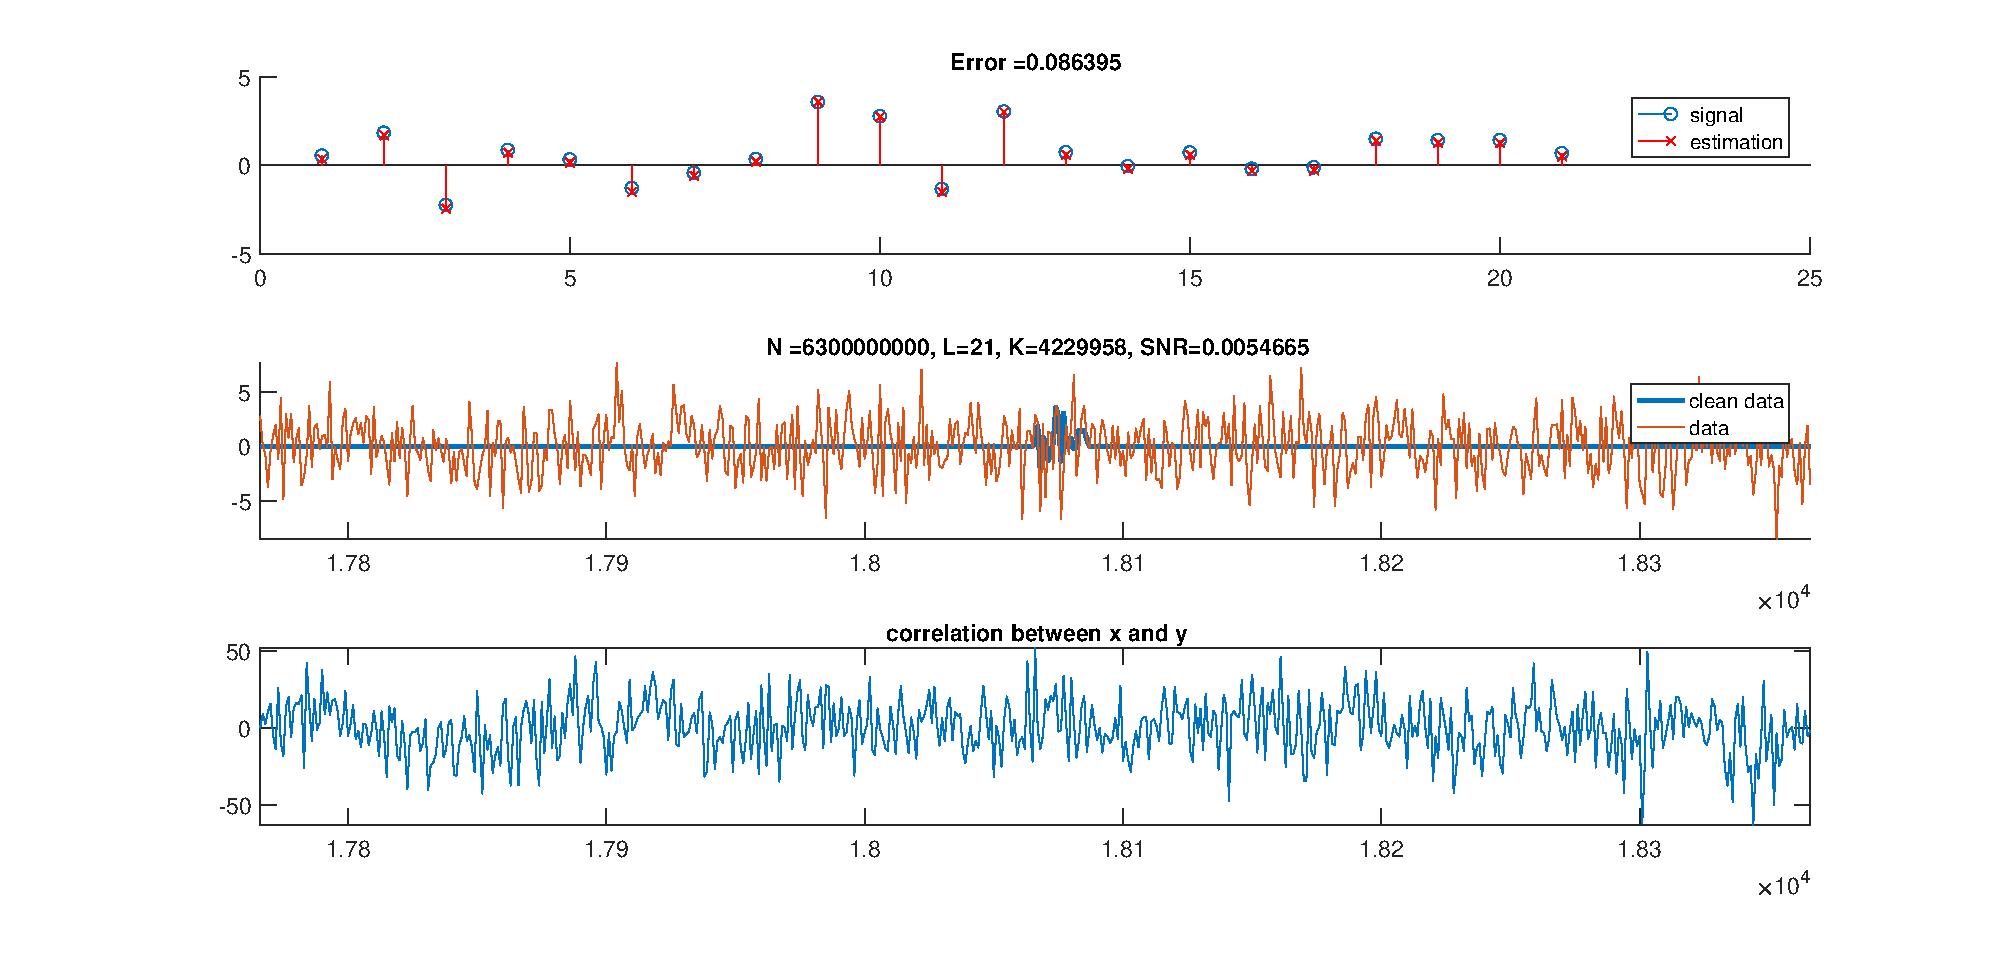
\includegraphics[scale=0.26]{example_random_signal.pdf}
	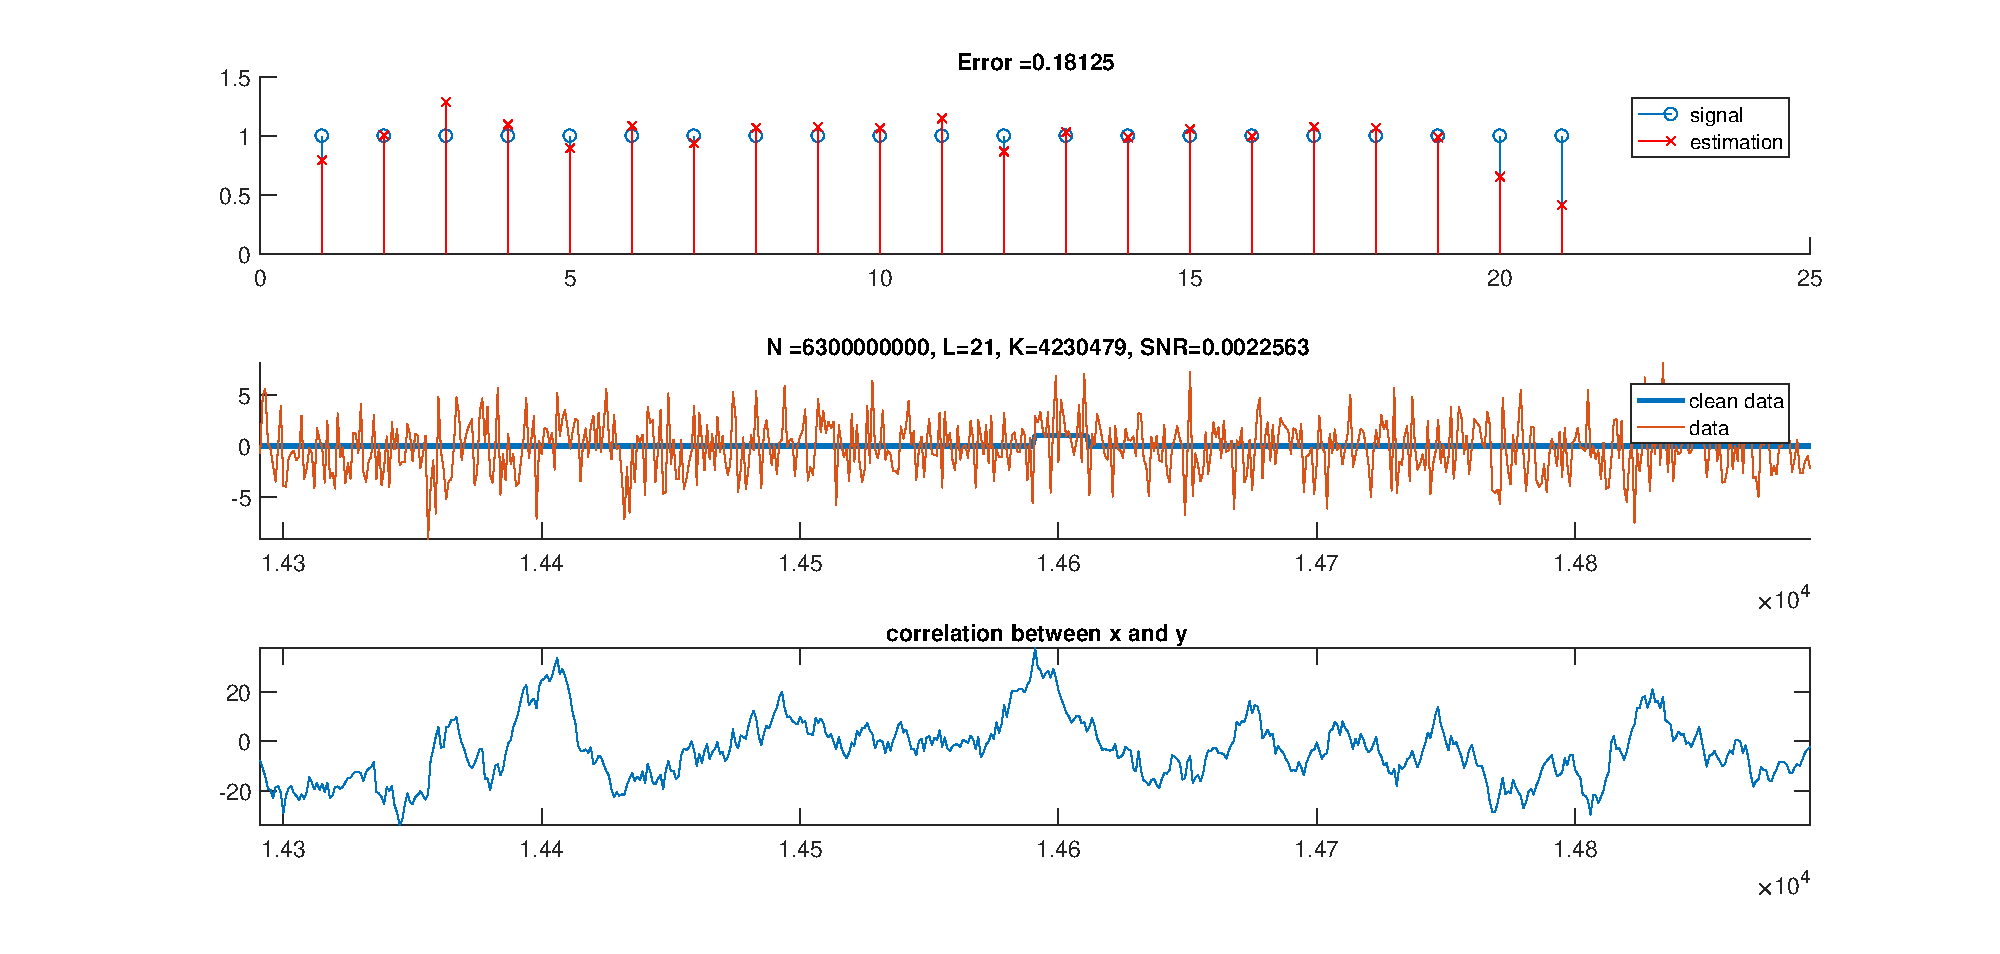
\includegraphics[scale=0.26]{example_rect_signal.pdf}	
	\caption{\label{fig:representative_example} Two representative examples of accurate estimation of an i.i.d./ random signal (left) and a rectangular signal (right), both of length $L=21$, from noisy measurements with $\sigma=2.5$ and $\SNR\approx 1/180$. The signal appearances $K=5\cdot 10^6$ times in the measurements of length $N=6WK$ for $W=10L$. The upper figure show the estimated signal versus the original one. Below that, we plot a typical segment of the noisy data. The bottom figures present a segment of the correlation between the underlying signals and the data.}
\end{figure*}


An experiment for constant noise level $\sigma=1$ and varying $k$ appears in Figure~\ref{fig:varyingK}. The error stops decreasing at some level from obvious reasons.


\begin{figure}
	\centering
	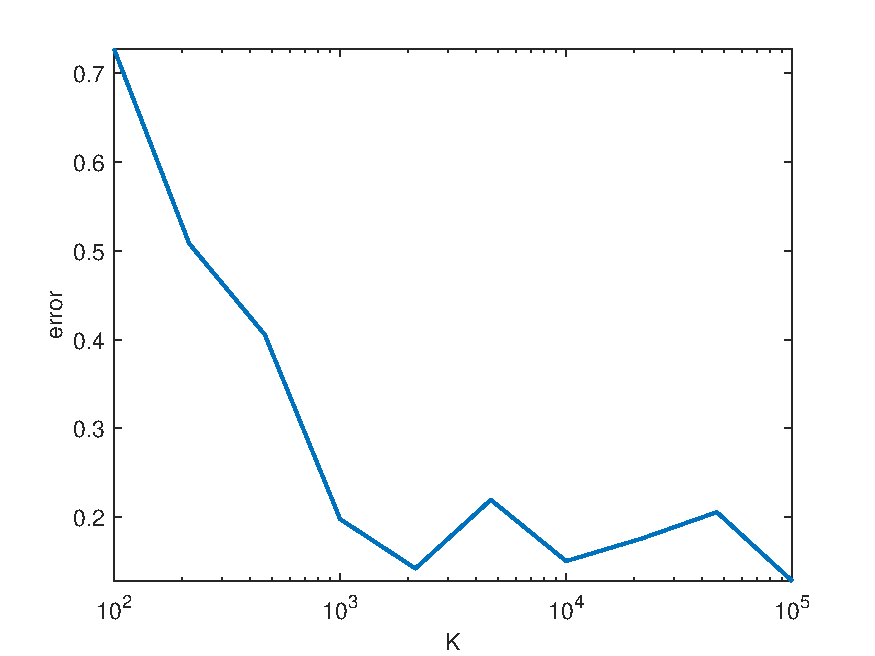
\includegraphics[scale=0.5]{errXP1.pdf}
	\caption{\label{fig:varyingK}The recovery error as a function of $k$, the number of signal appearances (approximately!) for $\sigma=1$. We worked with i.i.d.\ signal of length $L=1$ (same signal for all experiments), the window size was chosen as $W=10L$ and the number of measurements was chosen as $N =6Wk $. In average, $1/\SNR\approx 30$.}
\end{figure}



\section{Conclusion} \label{sec:conclusion}
Here we conclude the paper



\bibliographystyle{ieeetran}
\bibliography{ref}

\end{document}


 